\section{Results and discussion}
The number of fringes was plotted against the pressure change for the different gases and is found in Fig. \ref{fig:measurements}. As one can see in the figures all gases showed a linear relation which was expected. When comparing Fig. \ref{fig:Helium} with the others the number of fringes is a lot lower than for the others. This means that the index of refraction must be a lot lower for this and the relative error will probably be larger. 

\begin{figure}[H]
  \centering
  \begin{subfigure}{0.49\textwidth}
    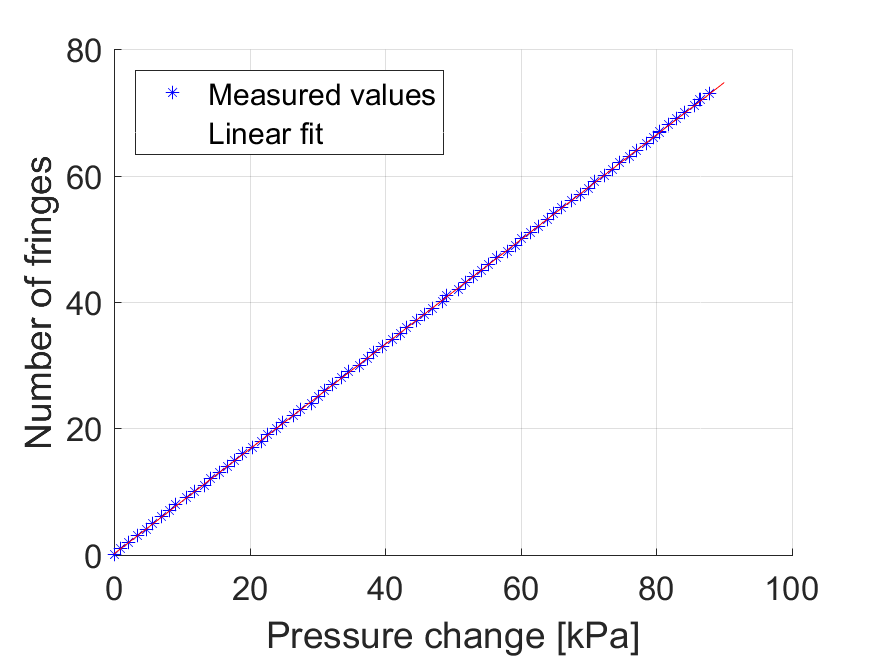
\includegraphics[width=\textwidth]{matlab/Air}
    \caption{Air}
    \label{fig:Air}
  \end{subfigure}
  \begin{subfigure}{0.49\textwidth}
    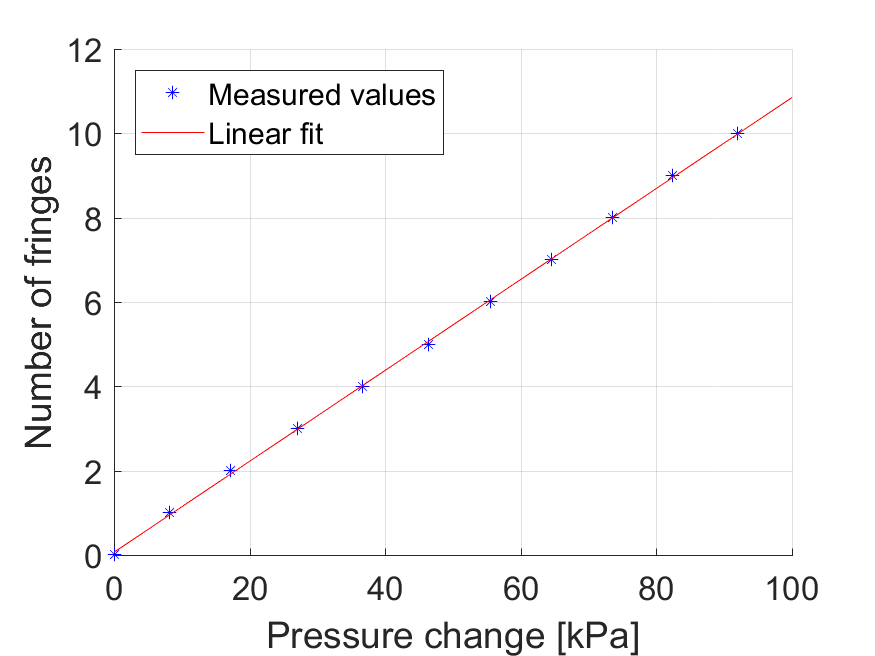
\includegraphics[width=\textwidth]{matlab/Helium}
    \caption{Helium}
    \label{fig:Helium}
  \end{subfigure}
  \begin{subfigure}{0.49\textwidth}
    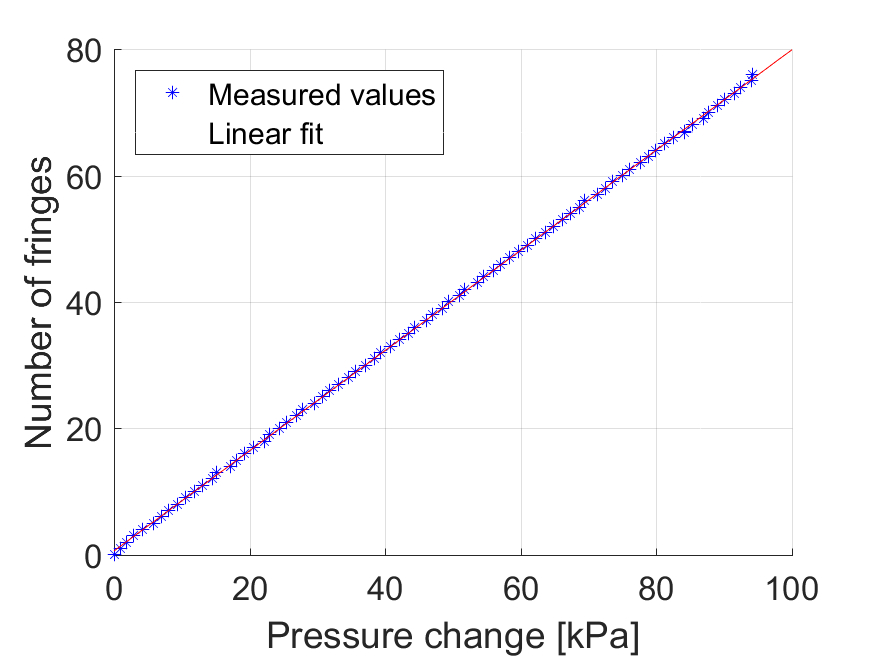
\includegraphics[width=\textwidth]{matlab/Argon}
    \caption{Argon}
    \label{fig:Argon}
  \end{subfigure}
  \begin{subfigure}{0.49\textwidth}
    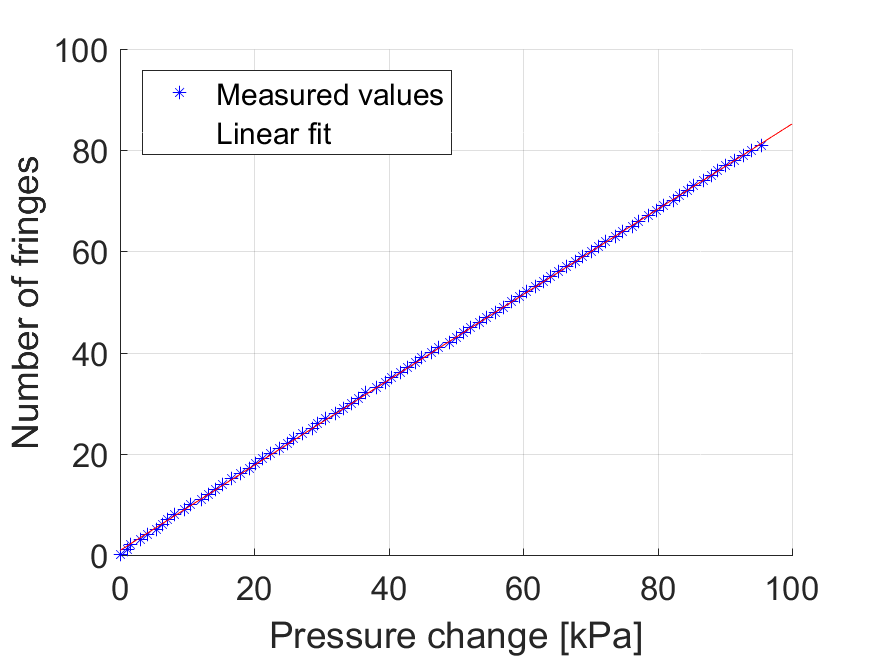
\includegraphics[width=\textwidth]{matlab/Nitrogen}
    \caption{Nitrogen}
    \label{fig:Nitrogen}
  \end{subfigure}
  \caption{Number of fringes and pressure change for the different gases with linear fits. Fitting parameters are found in Tab. \ref{tab:linearFits}}
  \label{fig:measurements}
\end{figure}

\begin{table}
  \centering
  \caption{Fitting parameters for the measured values in Fig. \ref{fig:measurements}. Linear fit on the form $y=\alpha x + \beta$.}
  \label{tab:linearFits}
  \begin{tabular}{l|l|l}
        & $\alpha$ & $\beta$ \\ \hline
  Air   & $0.828(1)$ kPa$^{-1}$ & 0.16(6) \\
  Helium & $0.108(1)$ kPa$^{-1}$ & 0.06(5) \\
  Argon  & $0.793(1)$ kPa$^{-1}$ & 0.61(5) \\
  Nitrogen & $0.843(1)$ kPa$^{-1}$ & 0.86(5)
  \end{tabular}
\end{table}
